\documentclass{standalone}
\usepackage[utf8]{inputenc}
\usepackage{braket}									
\usepackage{tikz}
\usepackage{tabularx}
\setlength{\extrarowheight}{-5pt}
\usetikzlibrary{arrows,positioning,shapes,backgrounds,fit}  
\usetikzlibrary{decorations.text}
\usetikzlibrary{decorations}
\usetikzlibrary{%
    decorations.pathreplacing,%
    decorations.pathmorphing%
}
\usepackage{pgfplots}
\pgfplotsset{width=8cm,compat=1.8}

\usepackage{amsmath}
\usepackage{xcolor}
\definecolor{DarkBlue}{rgb}{0.1,0.1,0.5}
\definecolor{Blue}{rgb}{0.1,0.1,0.8}
\definecolor{Red}{rgb}{0.75,0.,0.}
\definecolor{Gray}{gray}{0.3}
\definecolor{Green}{rgb}{0.2,0.5,0.2}
\newcommand*\circled[1]{\tikz[baseline=(char.base)]{
            \node[shape=circle,draw,inner sep=2pt] (char) {#1};}}
\begin{document}
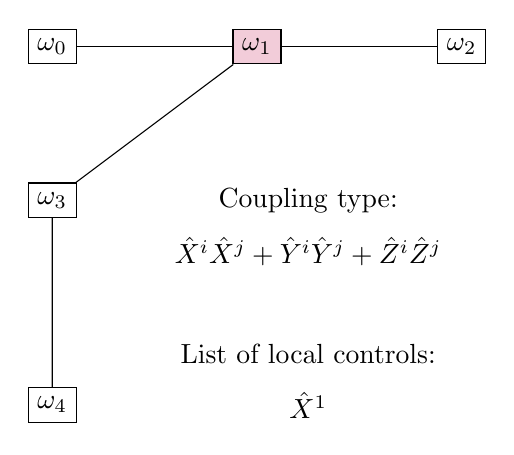
\begin{tikzpicture}[scale=1.3, wave/.style={
        decorate,decoration={snake,post length=1.4mm,amplitude=2mm,
        segment length=2mm},thick}]
   
\node[draw = black](p0) at (-2,0){$\omega_0$};
\node[ draw = black, fill=purple, fill opacity=0.2,text opacity=1](p1) at (0,0){$\omega_1$};
\node[ draw = black](p2) at (2,0){$\omega_2$};
\node[ draw = black](p3) at (-2,-1.5){$\omega_3$};
\node[ draw = black](p4) at (-2,-3.5){$\omega_4$};


\path[every node/.style={sloped,anchor=south,auto=false}]
(p0) edge    node { } (p1);
\path[every node/.style={sloped,anchor=south,auto=false}]
(p1) edge    node { } (p2);
\path[every node/.style={sloped,anchor=south,auto=false}]
(p1) edge    node { } (p3);
\path[every node/.style={sloped,anchor=south,auto=false}]
(p4) edge    node { } (p3);

\node[] at (0.5, -1.5) {Coupling type:};
\node[] at (0.5, -2) {$\hat{X}^i\hat{X}^j+\hat{Y}^i\hat{Y}^j+\hat{Z}^i\hat{Z}^j$};
\node[] at (0.5, -3) {List of local controls:};
\node[] at (0.5, -3.5) {$\hat{X}^1$};

%\node[] at (0.5, -4.5) {\begin{tabular}{ c c }
% Control type & Qubit \\\hline 
%   &   \\  
% $\hat{X}$ & 0 \\  
%$\hat{X}$ & 1 \\  
%$\hat{X}$ & 2 \\  
%$\hat{X}$ & 3 \\  
%$\hat{X}$ & 4 
%\end{tabular}};

\end{tikzpicture}

\end{document}

